
\documentclass[english]{article}

\pdfoutput=1

\usepackage[T1]{fontenc}
\usepackage[latin9]{inputenc}
\usepackage{verbatim}
\usepackage{float}
\usepackage{amsthm}
\usepackage{amsmath}
\usepackage{amssymb}
\usepackage{graphicx}
%\usepackage{multirow}
\usepackage{color}
\usepackage{url}
\usepackage{caption}
\usepackage{subcaption}


\newcommand{\TODO}[1]{{\color{red}{[#1]}}}

\makeatletter

%%%%%%%%%%%%%%%%%%%%%%%%%%%%%% Textclass specific LaTeX commands.
\numberwithin{equation}{section}
%\numberwithin{figure}{section}
\theoremstyle{plain}
\newtheorem{thm}{\protect\theoremname}[section]
\theoremstyle{definition}
\newtheorem{defn}[thm]{\protect\definitionname}
\theoremstyle{remark}
\newtheorem{claim}[thm]{\protect\claimname}
\theoremstyle{plain}
\newtheorem{lem}[thm]{\protect\lemmaname}

\newtheorem*{lem*}{Lemma}

\theoremstyle{remark}
\newtheorem{rem}[thm]{\protect\remarkname}
\theoremstyle{plain}
\newtheorem{corollary}[thm]{\protect\corollaryname}
\theoremstyle{plain}
\newtheorem{proposition}[thm]{\protect\propositionname}
%%%%%%%%%%%%%%%%%%%%%%%%%%%%%% User specified LaTeX commands.
%\usepackage{slashbox}

\usepackage{babel}
\providecommand{\claimname}{Claim}
\providecommand{\definitionname}{Definition}
\providecommand{\lemmaname}{Lemma}
\providecommand{\remarkname}{Remark}
\providecommand{\theoremname}{Theorem}
\providecommand{\corollaryname}{Corollary}
\providecommand{\propositionname}{Proposition}


\newcommand{\reals}{\mathbb{R}}
\newcommand{\RL}{\mathbb{R}^L}
\newcommand{\CL}{\mathbb{C}^L}
\newcommand{\RN}{\mathbb{R}^L}
\newcommand{\RNN}{\mathbb{R}^{N\times N}}
\newcommand{\CNN}{\mathbb{C}^{N\times N}}
\newcommand{\inner}[1]{\left\langle {#1} \right\rangle}
\newcommand{\hx}{\hat{x}} 

\newcommand{\SNR}{\textsf{SNR} } 

\begin{document}

\title{Estimation below the detection limit}


\author{Tamir Bendory}
\maketitle

\begin{abstract}
	Here comes the abstract
\end{abstract}

\section{Introduction}

In this paper, we consider the problem of estimating a set of signals $x_1,\ldots,x_K$ from their multiple occurrences in unknown, random, locations in the data $y$. The data may also contain background information -- independent of the signals -- which is model as noise.
For one-dimensional signals, the data can be thought of as a long time series and the signals as repetitive short events. For two-dimensional signals, the data is a big image that contains many smaller images.  
The problem is then to estimate the signals $x_1,\ldots x_K$ from $y$. This
model appears, in different noise levels, in many applications, including spike sorting~\cite{lewicki1998review}, passive radar~\cite{gogineni2017passive} and system identification~\cite{ljung1998system}.
In Section~\ref{sec:model} we provide a precise mathematical formulation of the problem.


If the noise level is negligible compared to the signal, the problem is easy.
One can detect the signal occurrences in the data, and then estimate the signals using clustering and averaging. However, in the low signal--to--noise (\SNR) regime, detection of individual signal occurrences is impossible as discussed in Section~\ref{sec:model}. Nonetheless, in Section~\ref{sec:autocorrelation} we show that under a separation condition on the signals occurrences and that $K$ is not too large, it is possible to estimate the signals, in any \SNR level, up to any desired accuracy.
This holds if each signals appears enough times in the data as will be explained next.

This work is primely motivated by the challenging innovative technologies for single particle reconstruction, such as cryo-electron microscopy (cryo--EM) and X-ray Free--Electron Laser (XFEL). The acquired data in these technologies suffers from very high noise level. Figure~\ref{fig:example} provides an example for the problem for one signal (i.e., $K=1$). Figures~\ref{fig:data2D_clean},\ref{fig:data2D_noisy_02} and~\ref{fig:data2D_noisy_1} shows excerpt of data in different noise levels, and~\ref{fig:signal2D_clean} is the underlying signal. Figure~\ref{fig:signal2D_LS} shows the estimation of the signal using our method when $\sigma=1$. In Section~\ref{sec:numerics}, after describing the model and method and detail, we provide the all details on this experiments and show more experiments for $K>1$.
In the last part of this manuscript, we will revisit the cryo--EM problem and draw connections with the estimation problem under consideration.

\begin{figure}[ht!]
    \advance\leftskip-4cm
   \advance\rightskip-4cm

%	\centering

	\begin{subfigure}{.5\textwidth}
		\centering
	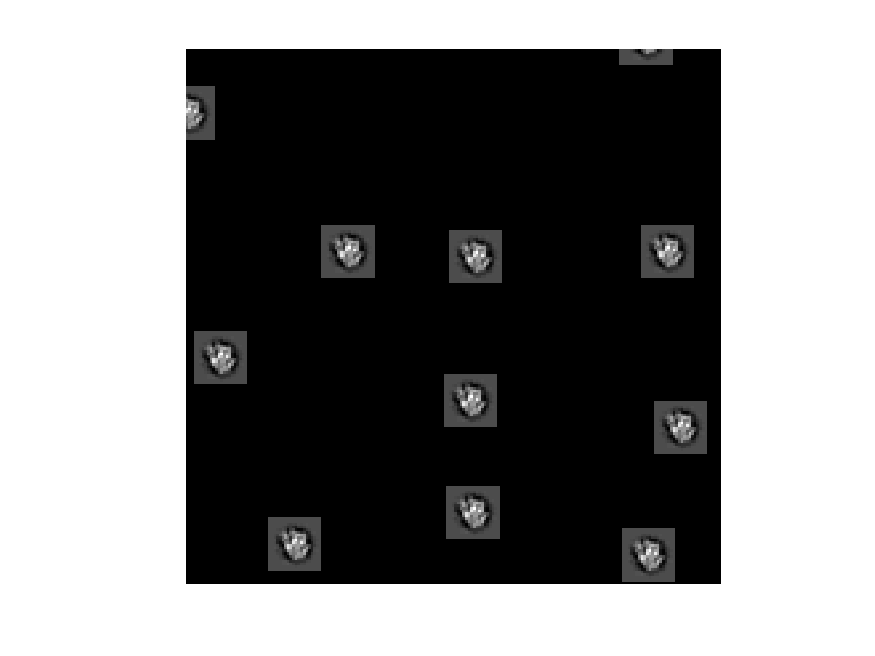
\includegraphics[scale=0.5]{data2D_clean}
\caption{Excerpt of clean data}
\label{fig:data2D_clean}
	\end{subfigure}%
	\begin{subfigure}{.5\textwidth}
	\centering
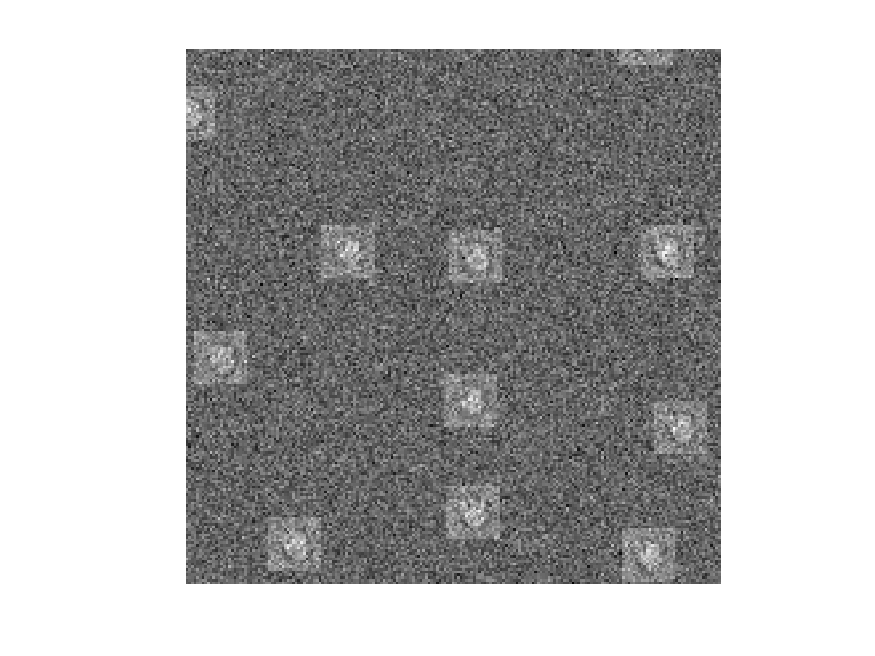
\includegraphics[scale=0.5]{data2D_noisy_02}
\caption{Excerpt of noisy data with $\sigma=0.2$}
\label{fig:data2D_noisy_02}
	\end{subfigure}
	\begin{subfigure}{.5\textwidth}
	\centering

\includegraphics[scale=0.5]{data2D_noisy_1}
\caption{Excerpt of noisy data with $\sigma=1$}
\label{fig:data2D_noisy_1}
\end{subfigure}

	\begin{subfigure}{.5\textwidth}
	\centering
	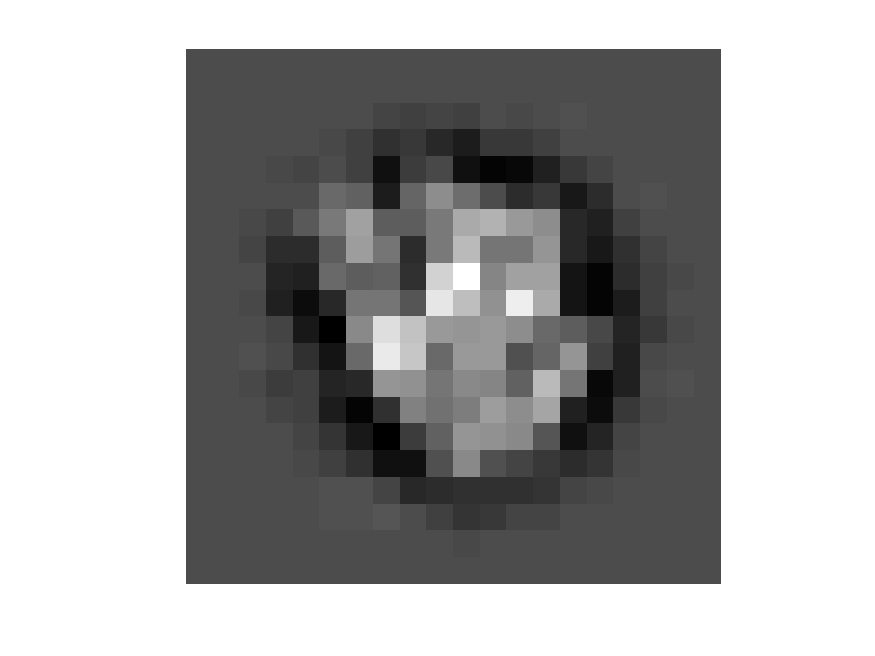
\includegraphics[scale=0.5]{signal2D_clean}
	\caption{Clean signal}
	\label{fig:signal2D_clean}
\end{subfigure}%
\begin{subfigure}{.5\textwidth}
	\centering
	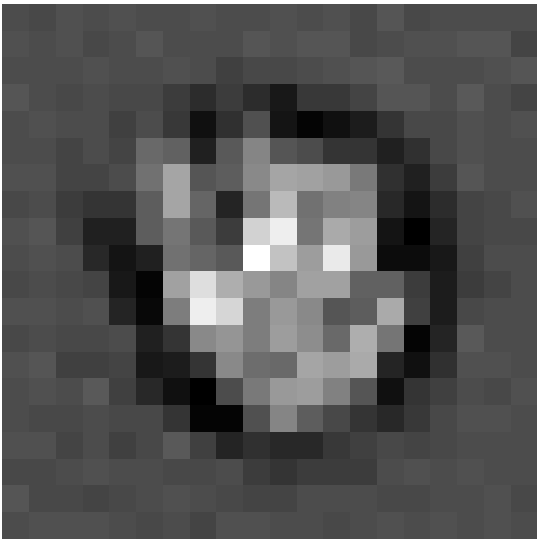
\includegraphics[scale=0.5]{signal2D_LS}
	\caption{Recovered signal using LS}
	\label{fig:signal2D_LS}
\end{subfigure}
\begin{subfigure}{.5\textwidth}
	\centering
	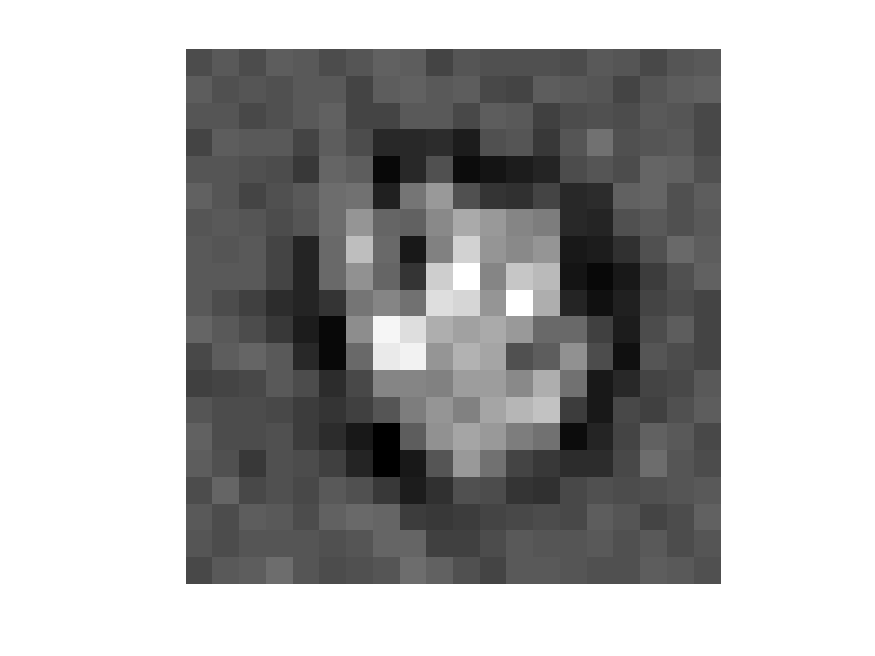
\includegraphics[scale=0.5]{signal2D_RRR}
	\caption{This one will be replaced}
	\label{fig:signal2D_RRR}
\end{subfigure}

\caption{Example}
\label{fig:example}
\end{figure}

In Section~\ref{sec:autocorrelation}, we elaborate on our method to
estimate the signal in the low \SNR regime using autocorrelation analysis. In a nutshell,
the method consists of two stages. First, we estimate a mix of the low order autocorrelations of the signals from the data. These quantities can
be estimated to any desired accuracy if the signals appear enough times in the measurements, without the need to detect individual occurrences. Then, the signals are estimated from the mixed autocorrelations. Interestingly, alternative methods which are often employed in similar estimation problems, such as expectation-maximization (EM) or Monte-Carlo Markov Chain (MCMC), seems to be intractable for this problem. 


\section{Model}  \label{sec:model}

Let $x_1,\ldots,x_K\in\RL$ be the sought signals and let $y\in\RN$ be the measurement. For each $x_i$, let $s_i\in\{0,1\}^N$ be a binary signal, referred to as the \emph{support signal}. The non-zero values of $s_i$ indicates the locations of $x_i$ in $y$. If $s_i[n]=1$, then $y[n+j] = x_i[n+j]+\varepsilon[n+j]$ for $j=0,\ldots,L-1$. The further denote $s = \sum_{i=1}^Ks_i$ as the union of supports. 

The support signals are generated by the following generative model. First, an index $i_1$ is drawn uniformly from $\{1,\ldots,N\}$. A second index $i_2$ is drawn uniformly from $\{1,\ldots,N\}$. If $\vert i_2-i_1\vert \geq L-1$,
then we set $s[i_2]=1$, otherise we keep $s[i_2]=0$ and draw an index again. We proceed to add non-zero entries to $s$ while keeping the separation condition. This process is halted when the number of when support is full enough by some predefined criterion. Once the signal $s$ is determined, for each non-zero entries is drawn from $\{1,\ldots,K\}$ and associated with the chosen signal. We note that if the support is sparse enough, this generative model can be approximated by a simpler process that ignores the separation constraint and simply choose $m$ random location in uniform over $\{1,\ldots N\}$. The number of occurrences $m_i,\ldots,m_K$ is unknown to us. 

The simplest way to present the forward model is a blind deconvolution problem between the support signals and the unknown signals
\begin{equation}
y = \sum_{i=1}^K x_i\ast s_i + \varepsilon,\quad \varepsilon\sim\mathcal{N}(0,\sigma^2 I).
\end{equation}
We model the background information as i.i.d.\ Gaussian noise with zero mean and $\sigma^2$ variance. 
The goal is to estimate $x1,\ldots,x_K$ from $y$.

Blind deconvolution is a longstanding problem, arising in a variety of engineering and scientific applications, such as astronomy, communication, image deblurring, system identification and optics; see~\cite{jefferies1993restoration,shalvi1990new,ayers1988iterative,abed1997blind}, just to name a few. Clearly, without additional information on the signal, blind deconvolution is ill-posed. In our case, the prior information is that $s$ is a binary, sparse, signal. 
Other settings of blind deconvolution problems have been analyzed recently under different settings, see for instance~\cite{ahmed2014blind,li2016identifiability,li2016rapid,ling2015self,ling2017blind,chi2016guaranteed}
where the focus is on the high \SNR regime.

If $x$ is known and $K=1$, then  $s$ can be estimated by linear program in high \SNR~\cite{de2012exact,duval2015exact,bendory2016robust,bendory2017robust,bernstein2017deconvolution}. However, in the low \SNR regime, estimating $s$ is impossible. To see that, suppose that for each non-zero value of $s$, an oracle provides you 
a window that contains it. Namely, we get a series of windows, each one contains a signal at unknown location. The question is whether one can estimate the locations of the signals within the windows. Apparently, this cannot be done. For instance, the variance of any estimator is, at best, proportional to $\sigma^2$ and independent of the number of windows, even if $x$ is known~\cite{aguerrebere2016fundamental}.  Since this alignment problem is essentially easier then the problem under consideration, we conclude that detecting the non-zero values of $s$ is impossible in low \SNR. In our setup, $s$ is the \emph{latent} variable of the problem. Indeed, in many blind deconvolution applications the goal is merely to estimate one of the unknown signals. For instance, in image deblurring, both the blurring
kernel and the high-resolution image are unknown, but the prime goal is only
to sharpen the image.
In the next section we show that if $M$ is large enough, then estimating the signals is possible, in any \SNR level and to any accuracy, although we cannot estimate their occurrences. 



\section{Autocorrelation analysis}   \label{sec:autocorrelation}



\section{Numerical experiments}   \label{sec:numerics}


\bibliographystyle{plain}
\bibliography{ref}

\end{document}

